\documentclass{beamer}
\usepackage[utf8]{inputenc}
\usepackage[T1]{fontenc}
\usepackage{listings}

\lstset{basicstyle=\scriptsize\ttfamily,breaklines=true}
\lstset{framextopmargin=50pt,frame=bottomline}

\title{Patching Binaries to Improve Fuzzing}
\date{\today}
\author[Eubanks]{Alex Eubanks \texttt{<alex.eubanks@forallsecure.com>}}

\usetheme{fas}

\begin{document}

\begin{frame}
\titlepage
\end{frame}

\section{Agenda}

\begin{frame}{Agenda}
\setlength{\parskip}{0cm}
\tableofcontents
\end{frame}

\section{Introduction}

\begin{frame}
\frametitle{Introduction}
In this tutorial, we will learn how to modify binary applications to improve the
fuzzing process. If source code is available, there is never a reason to modify
a binary. Make the necessary changes in source, and recompile your binary for
testing.\par
When testing of 3rd-party, or legacy applications, is required, source code may
not be available. Binary patching can be used to improve the speed and
efficiency of testing these programs with MAYHEM.
\end{frame}

\subsection{Requirements}

\begin{frame}
\frametitle{Requirements}
\begin{itemize}
  \item A working copy of MAYHEM, with the mayhem client installed on the 
    command line.
  \item Reverse-engineering expertise. This is an advanced tutorial, and you
    should be comfortable with assembly-level code.
  \item A disassembler with the ability to patch instructions. We will be using
    Binary Ninja\footnote{https://binary.ninja}.
  \item The example files that are referenced throughout the slide deck.
\end{itemize}
\end{frame}

\subsection{Why Patch Binaries}
\begin{frame}
\frametitle{Why Patch Binaries}
Binary modification is not required for fuzzing, but there are several reasons
why vulnerability researchers sometimes modify binaries. Some example reasons:

\begin{itemize}
  \item Allow a program to cleanly exit after running a single testcase.
  \item Remove checksum checks that some input-generation tools are not aware
    of.
  \item Remove cryptographic primitives from a binary.
  \item Remove irritating program behaviors that disrupt fuzzing.
\end{itemize}

In general, we want to remove checks that an attacker can create themselves, but will cause a program to exit before exercising code paths. A common example is a checksum over an incoming data stream.
\end{frame}

\subsection{Example Scenarios}

\begin{frame}
\frametitle{A Checksum Story}
Checksums can be disruptive to fuzzing. They cause applications to dismiss input
which may otherwise trigger a bug. Attackers will checksum their malicious data
before feeding it to your applications, so we shouldn't allow checksums over
input data to slow down our analysis.
\par
If we fail to account for this checksum, each time MAYHEM generates a testcase
with a bad checksum, it will be thrown out. There are two basic ways to
account for this checksum:

\begin{itemize}
  \item We can pass our inputs through a harness, which will ensure proper
    checksums are in place before passing those inputs to the program under
    test.
  \item We can patch the binary so that it accepts all inputs, even those with
    invalid checksums.
\end{itemize}

We will explore the second option in this tutorial.
\end{frame}

\section{A Checksum Story: Imagemagick}

\begin{frame}
\frametitle{A Checksum Story: Imagemagick}
In this example, we are going to fuzz png parsing in a popular command-line
image-manipulation program called
"imagemagick"\footnote{https://www.imagemagick.org/}.
\par
Imagemagick is an opensource, freely available application with source. Normally
we would recommend you make any necessary modifications in source, but we will
be dismissing source code and working directly with the binary for this
tutorial.
\end{frame}


\subsection{Getting set up with Imagemagick}
\begin{frame}[fragile]
\frametitle{Getting set up with Imagemagick}
Let's start from a fresh Debian Stretch linux environment, and install
imagemagick directly from the package repositories.
  \begin{lstlisting}
apt-get update && \
apt-get dist-upgrade -y && \
apt-get install -y imagemagick
  \end{lstlisting}

And let's run imagemagick over an image:
  \begin{lstlisting}
$ convert /tutorials/binary-patching/imagemagic/nsa-insignia-sm.png -enhance /tutorials/binary-patching/imagemagic/enhanced.png
$
  \end{lstlisting}

No errors, Perfect!
\end{frame}


\begin{frame}[fragile]
\frametitle{Getting set up with Imagemagick}
Knowing that the PNG file format uses crc checksums, I've created a modified PNG
which causes imagemagic to print out failed checksum errors. I did this by
running radamsa\footnote{https://github.com/aoh/radamsa} over our
\texttt{nsa-insignia-sm.png} file, and testing the output until I had a new PNG
that gave an error for invalid checksum.
\par
  \begin{lstlisting}
root@a67f5575a117:~# convert /tutorials/binary-patching/imagemagic/nsa-insignia-crc-error.png /tmp/out.png
convert-im6.q16: IDAT: CRC error `/tutorials/binary-patching/imagemagic/nsa-insignia-crc-error.png' @ error/png.c/MagickPNGErrorHandler/1628.
root@a67f5575a117:~# 
  \end{lstlisting}

We can see the CRC error, which is exactly what we want. Perfect!
\end{frame}


\subsection{Finding the CRC Check}

\begin{frame}
\frametitle{Finding the CRC Check}
We now need to find the code which is performing this CRC check, and remove it
by patching the binary.
\par
There are a couple ways we can move forward. We can:

\begin{itemize}
  \item Search for magic numbers associated with the algorithm we are trying to
    modify, and work backwards to see where the output of that algorithm is
    verified against our input.
  \item Use the strings in the error message to find the relevant code.
  \item Reverse-engineer the binary until we find the correct place to patch.
\end{itemize}

Since we have strings in an error message, let's start with those and see if we
can find out how to patch around this crc check.
\end{frame}


\begin{frame}[fragile]
\frametitle{Finding the "CRC Error" string}
We'll start by using our good friend \texttt{grep} to find the string
"CRC error".

\begin{lstlisting}
root@a67f5575a117:~# grep "CRC error" /usr/bin/convert
root@a67f5575a117:~# 
\end{lstlisting}

Not in the convert binary... Let's take a look at the dependencies on the next
slide.
\end{frame}


\begin{frame}[fragile]
\frametitle{Listing dependencies}
\begin{lstlisting}[breaklines=false]
root@a67f5575a117:~# ldd /usr/bin/convert
linux-vdso.so.1 (0x00007ffec85d3000)
libMagickCore-6.Q16.so.3 => /usr/lib/x86_64-linux-gnu/libMagickCore-6.Q16.so.3 (0x00007f2a0215a000)
libMagickWand-6.Q16.so.3 => /usr/lib/x86_64-linux-gnu/libMagickWand-6.Q16.so.3 (0x00007f2a01e31000)
libpthread.so.0 => /lib/x86_64-linux-gnu/libpthread.so.0 (0x00007f2a01c14000)
...
libglib-2.0.so.0 => /lib/x86_64-linux-gnu/libglib-2.0.so.0 (0x00007f29ff535000)
libexpat.so.1 => /lib/x86_64-linux-gnu/libexpat.so.1 (0x00007f29ff30b000)
libpng16.so.16 => /usr/lib/x86_64-linux-gnu/libpng16.so.16 (0x00007f29ff0d8000)
libxcb.so.1 => /usr/lib/x86_64-linux-gnu/libxcb.so.1 (0x00007f29feeb0000)
...
libbsd.so.0 => /lib/x86_64-linux-gnu/libbsd.so.0 (0x00007f29fe419000)
librt.so.1 => /lib/x86_64-linux-gnu/librt.so.1 (0x00007f29fe211000)
\end{lstlisting}

\texttt{libpng16.so.16}, this looks interesting.
\end{frame}


\begin{frame}[fragile]
\frametitle{Finding the "CRC error" string}
Let's search for the string in \texttt{/usr/lib/x86\_64-linux-gnu}, where most
of our dependencies reside.

\begin{lstlisting}
root@a67f5575a117:~# grep "CRC error" /usr/lib/x86_64-linux-gnu/*                       
...
Binary file /usr/lib/x86_64-linux-gnu/libpng16.so.16 matches
Binary file /usr/lib/x86_64-linux-gnu/libpng16.so.16.28.0 matches
...
\end{lstlisting}

It looks like we need to patch \texttt{libpng16.so.16.28.0}. Your linux
distribution may have a different version of libpng, but you should be fine to
play along with whichever version you have.
\par
Let’s open \texttt{libpng16.so.16.28.0} in Binary Ninja.
\end{frame}

\begin{frame}
\frametitle{Libpng in Binary Ninja}
  \small{Here we have the libpng library open in Binary Ninja.}
  \begin{tikzpicture}
  \node[inner sep=0pt]
    {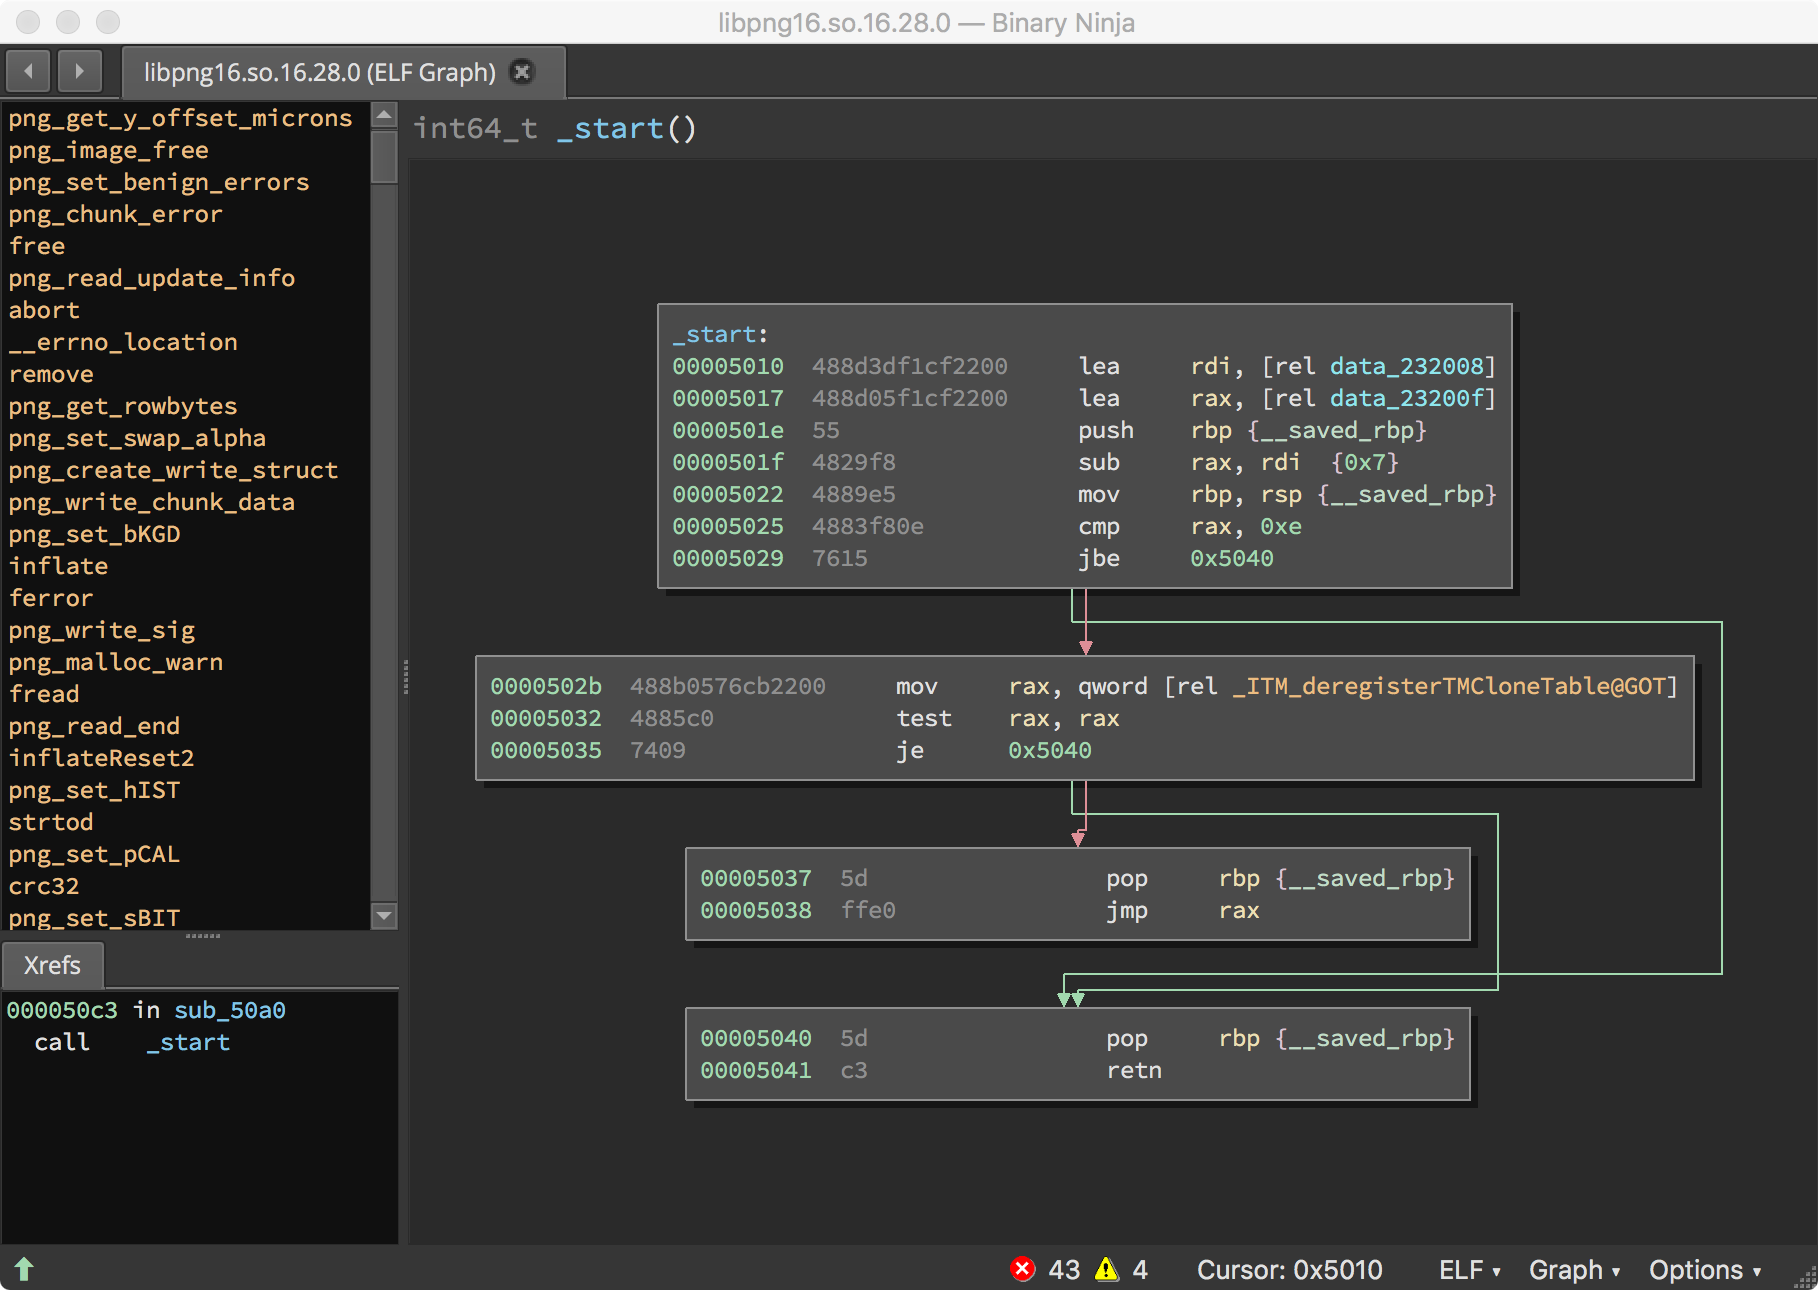
\includegraphics[width=1\textwidth]{images/imagemagick-binary-ninja-0.png}};
  \end{tikzpicture}
\end{frame}

\note{A view of libpng opened in Binary Ninja}

\begin{frame}
\frametitle{Libpng in Binary Ninja}
  \small{We begin searching for "CRC error". It looks like we found a
    substring.}
  \begin{tikzpicture}
  \node[inner sep=0pt]
    {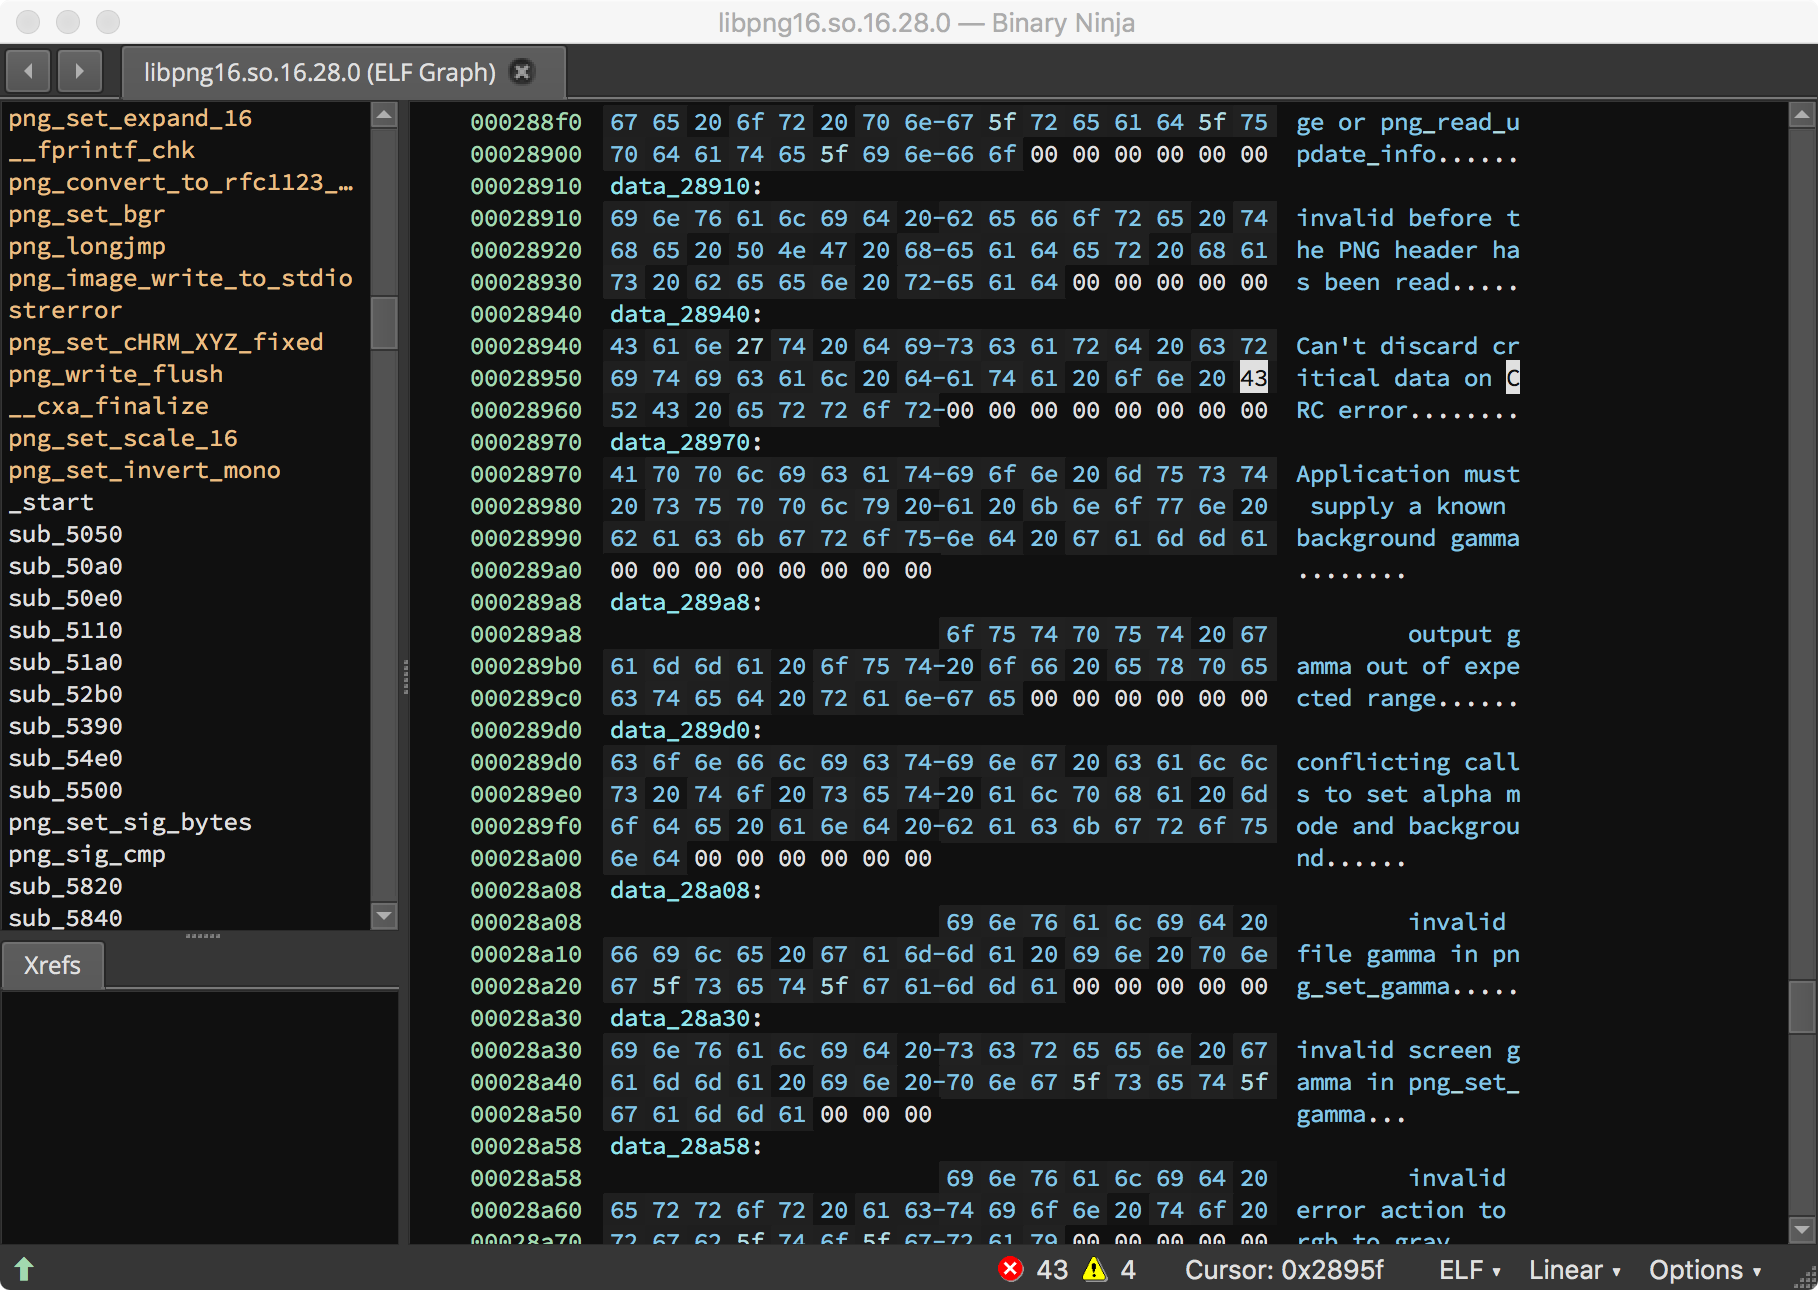
\includegraphics[width=1\textwidth]{images/imagemagick-binary-ninja-1.png}};
  \end{tikzpicture}
\end{frame}

\begin{frame}
\frametitle{Searching for "CRC error"}
  \small{It looks like we've found the right "CRC error" string. Follow the Xref
    in the bottom-left corner}
  \begin{tikzpicture}
  \node[inner sep=0pt]
    {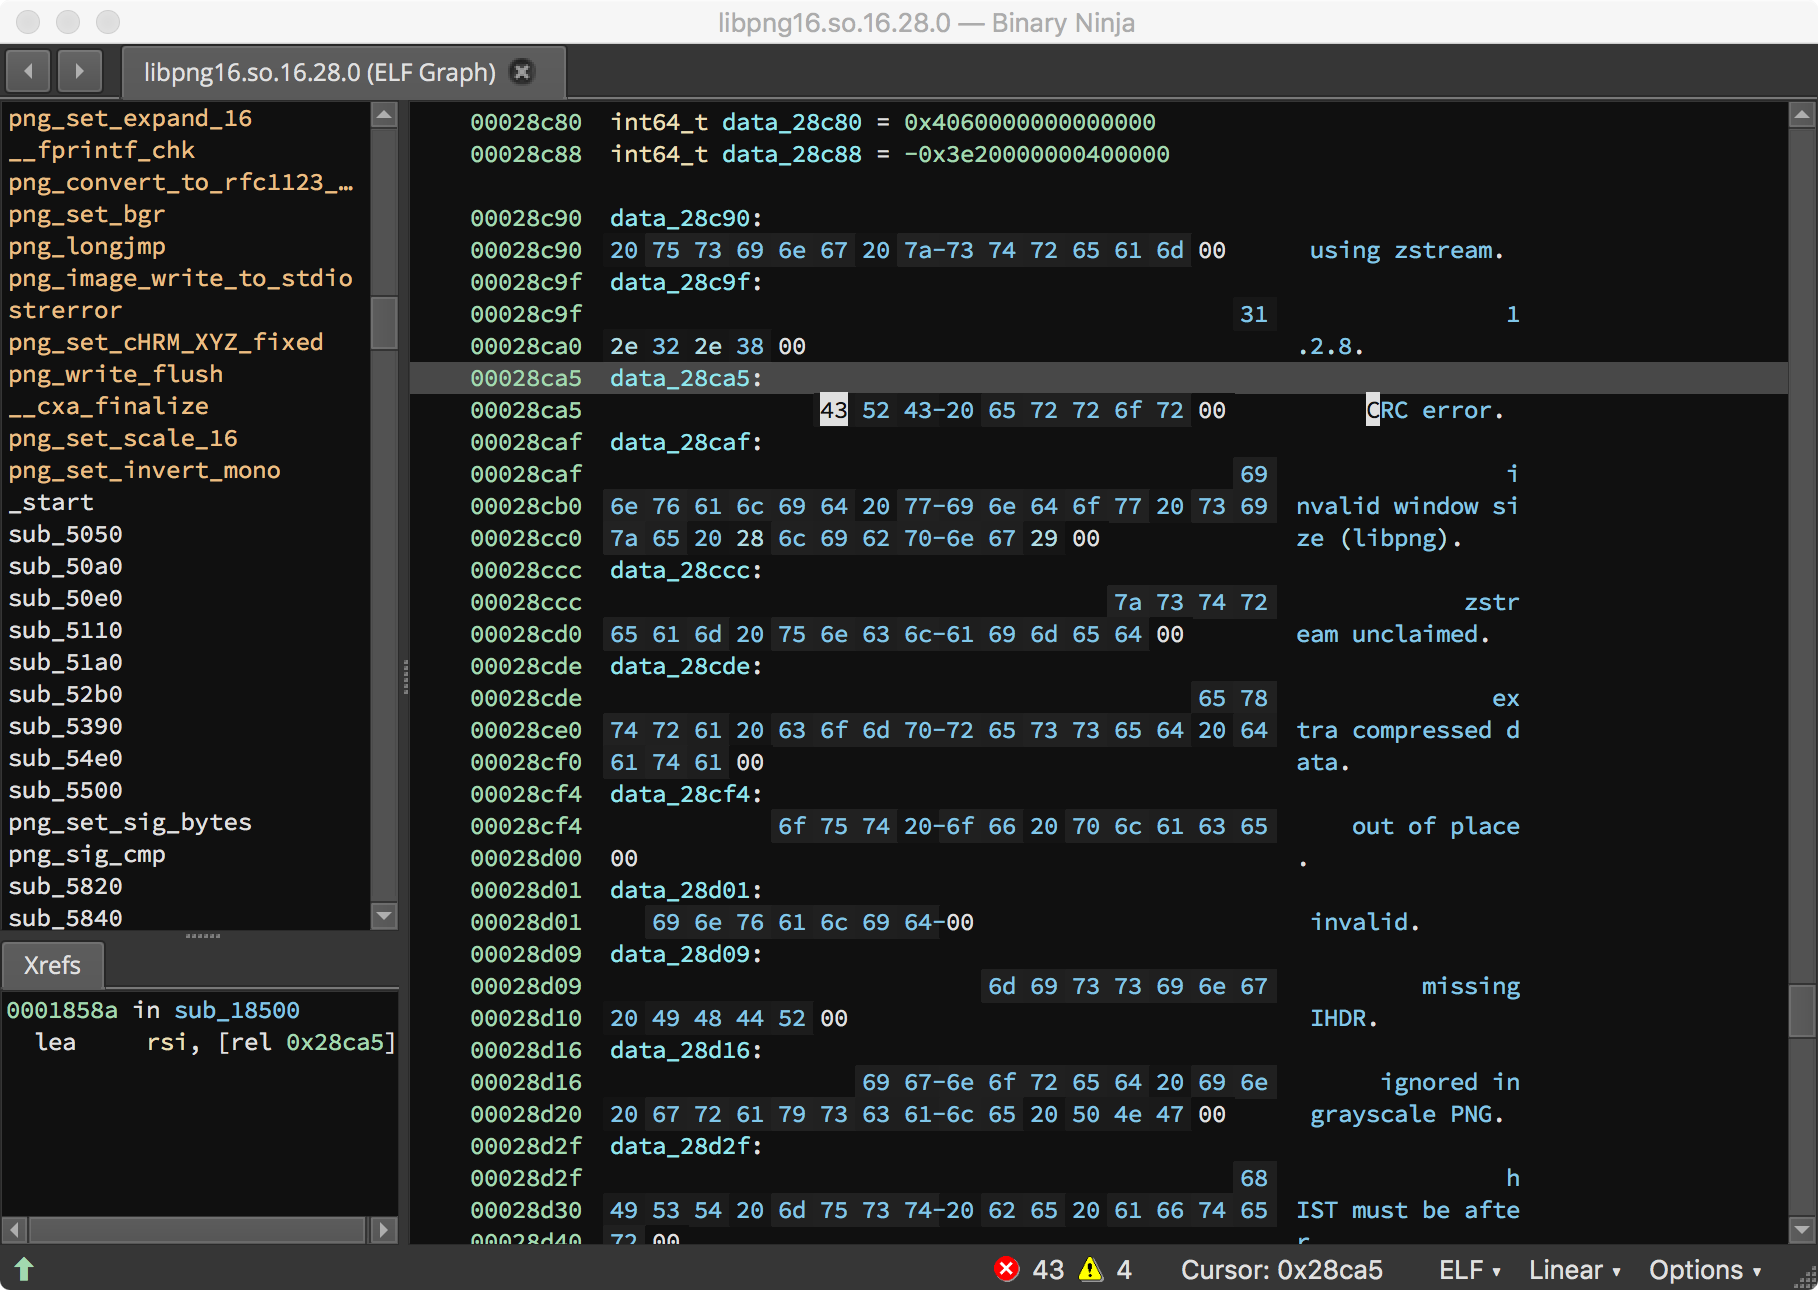
\includegraphics[width=1\textwidth]{images/imagemagick-binary-ninja-2.png}};
  \end{tikzpicture}
\end{frame}

\subsection{Modifying libpng}

\begin{frame}
\frametitle{Patching out the CRC check}
  \begin{tikzpicture}
  \node[inner sep=0pt]
    {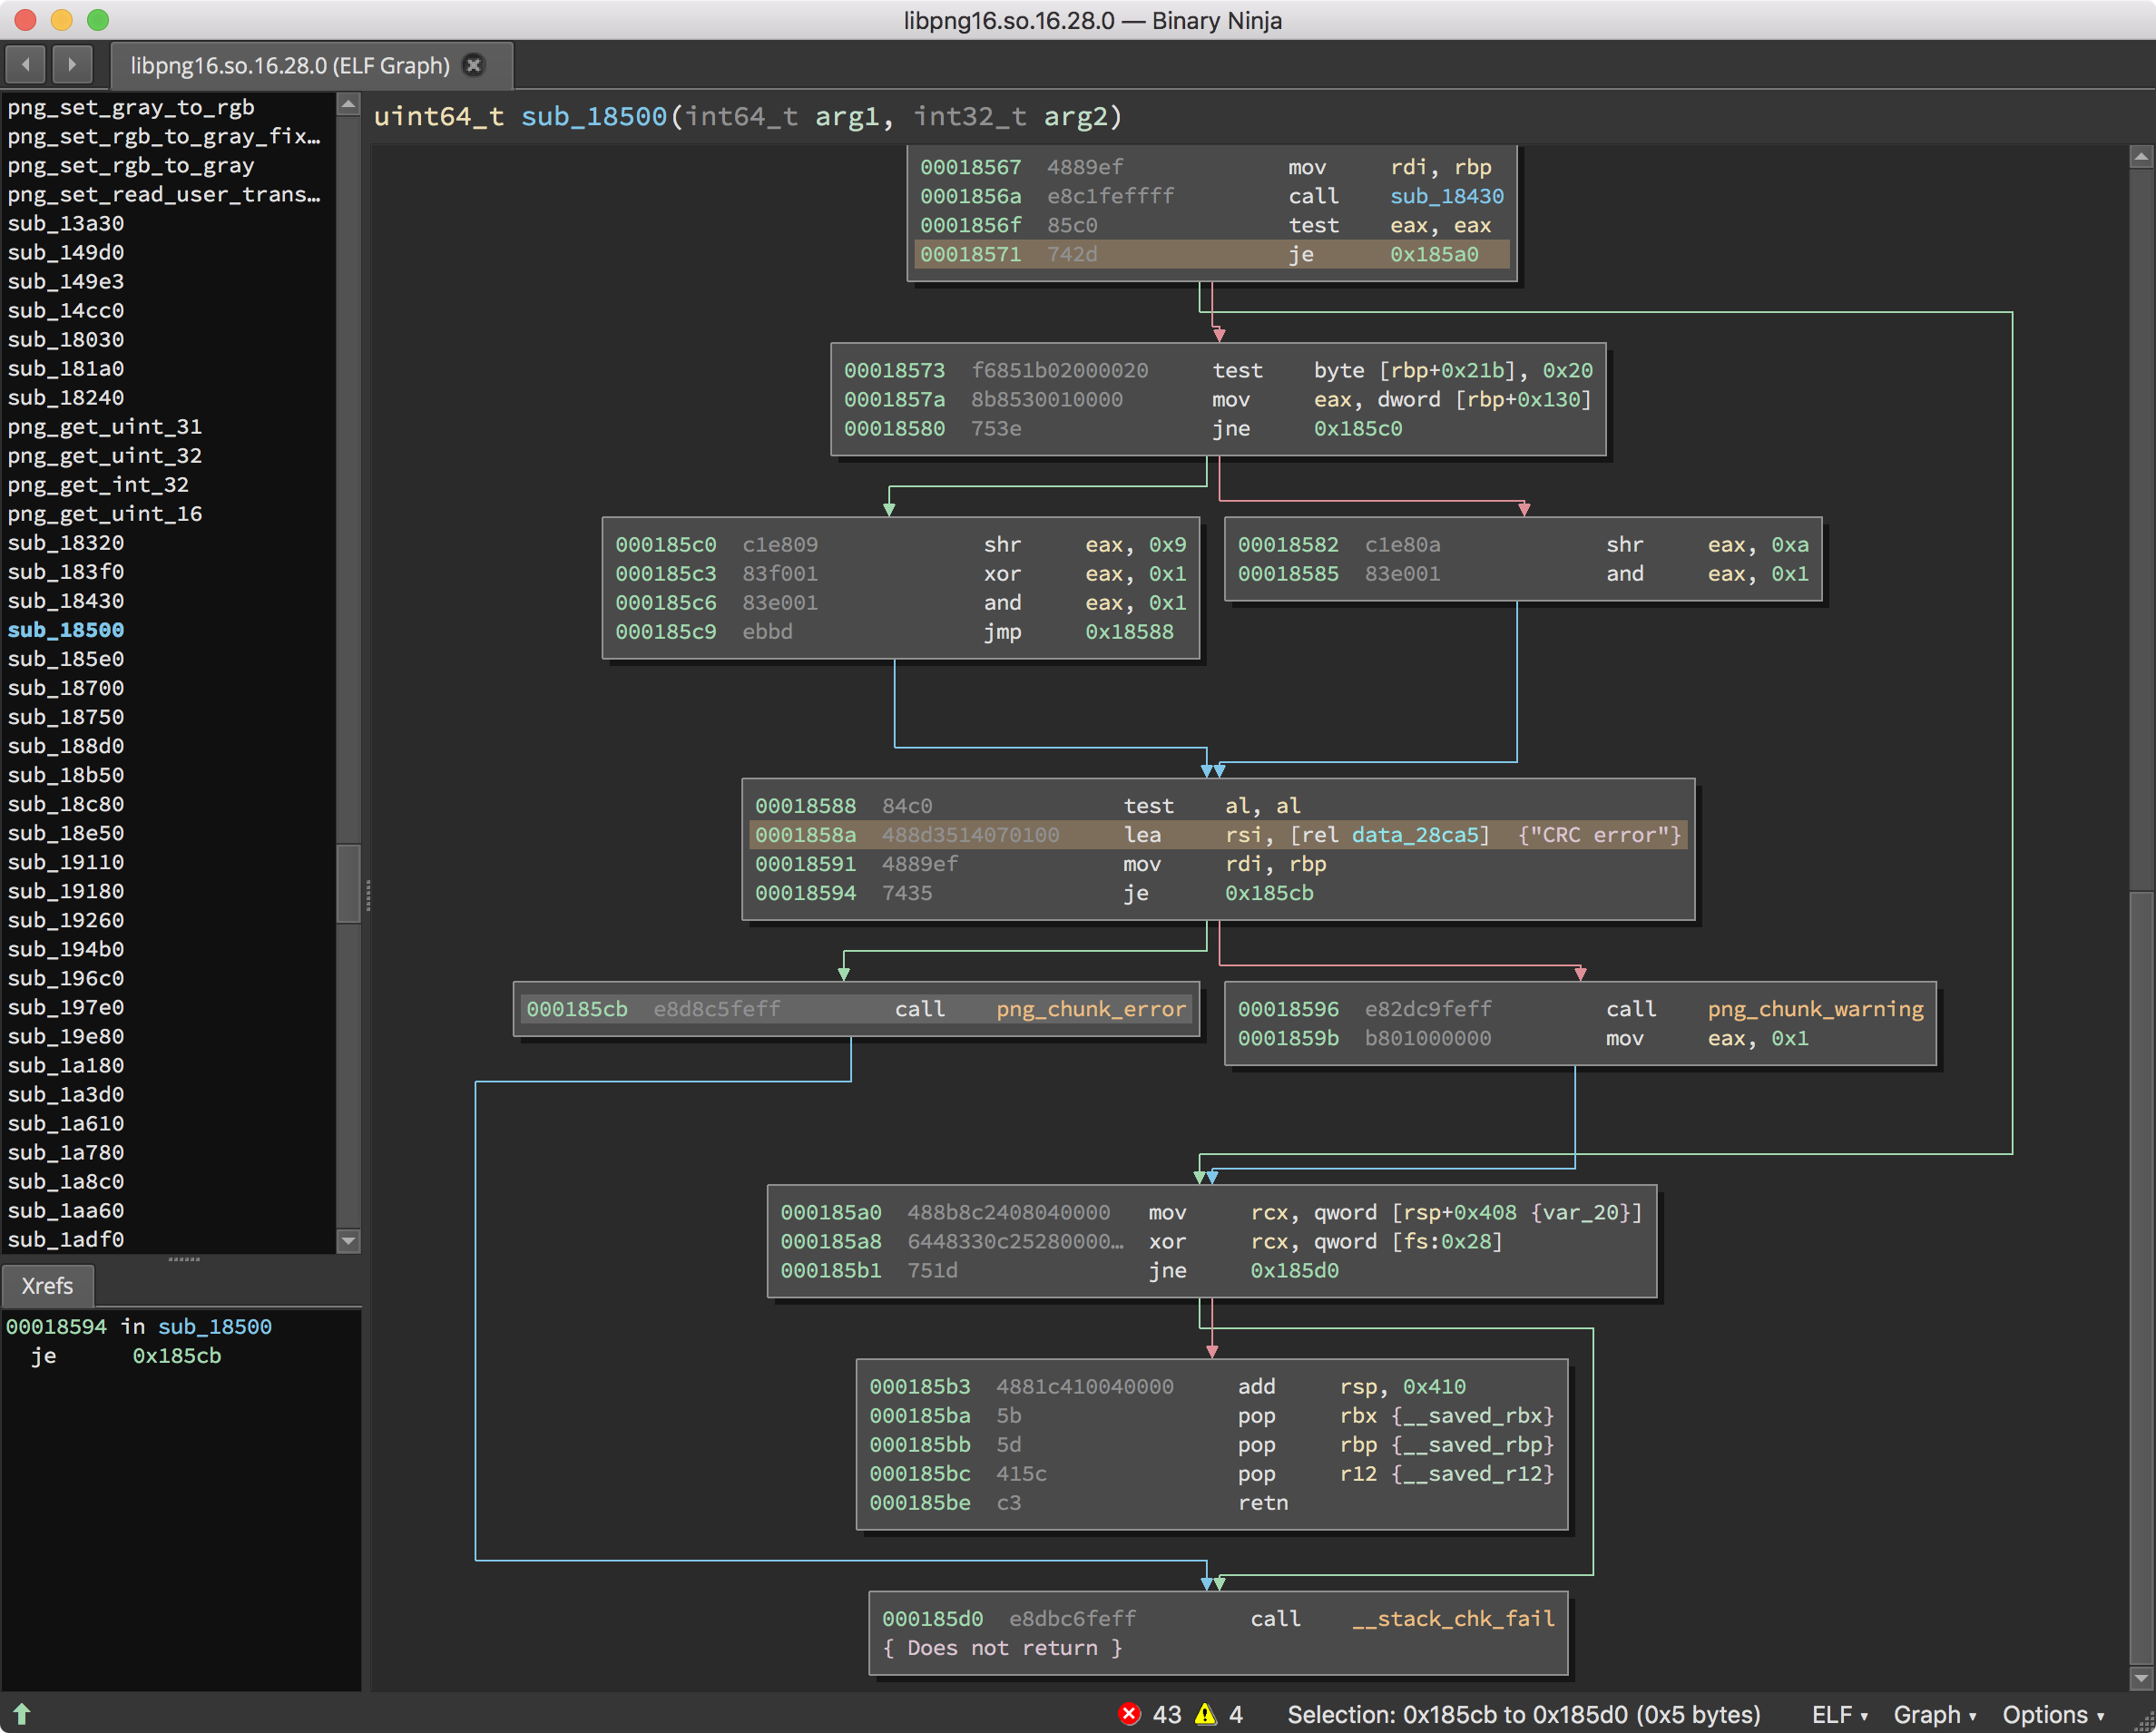
\includegraphics[width=1\textwidth]{images/imagemagick-binary-ninja-3.png}};
  \end{tikzpicture}
\end{frame}

\begin{frame}
\frametitle{Patching out the CRC check}
A quick look at this function shows our "CRC error" string being loaded
immediately prior to a call to \texttt{png\_chunk\_error} or
\texttt{png\_chunk\_warn}. We hope all we need to do is avoid the blocks which
drive us over \texttt{png\_chunk\_error} and \texttt{png\_chunk\_warn}.
\par
If we can always take the branch at \texttt{0x18571}, hopefully we can avoid
libpng dying on checksum errors, and we will be able to more efficiently fuzz
imagemagick.
\end{frame}

\begin{frame}
\frametitle{Libpng in Binary Ninja}
  Right-click the instruction at \texttt{0x18571}, and choose
  \texttt{Patch -> Always Branch}.
  \begin{tikzpicture}
  \node[inner sep=0pt]
    {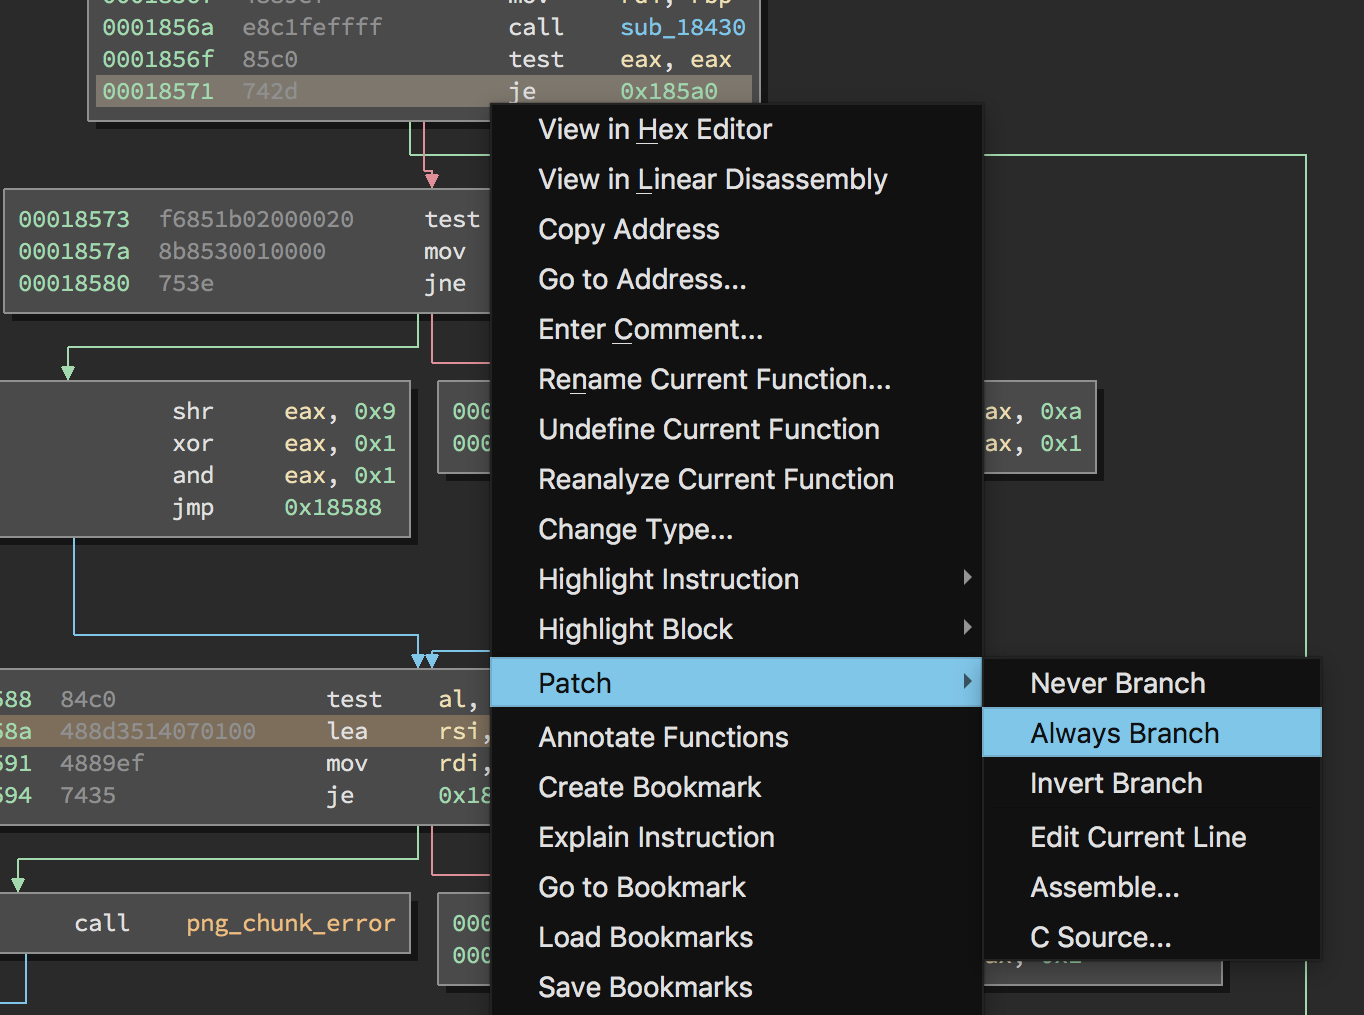
\includegraphics[width=1\textwidth]{images/imagemagick-binary-ninja-4.png}};
  \end{tikzpicture}
\end{frame}

\begin{frame}
\frametitle{Libpng in Binary Ninja}
  \small{Our patched libpng binary, with errors on CRC mismatches removed.}
  \begin{tikzpicture}
  \node[inner sep=0pt]
    {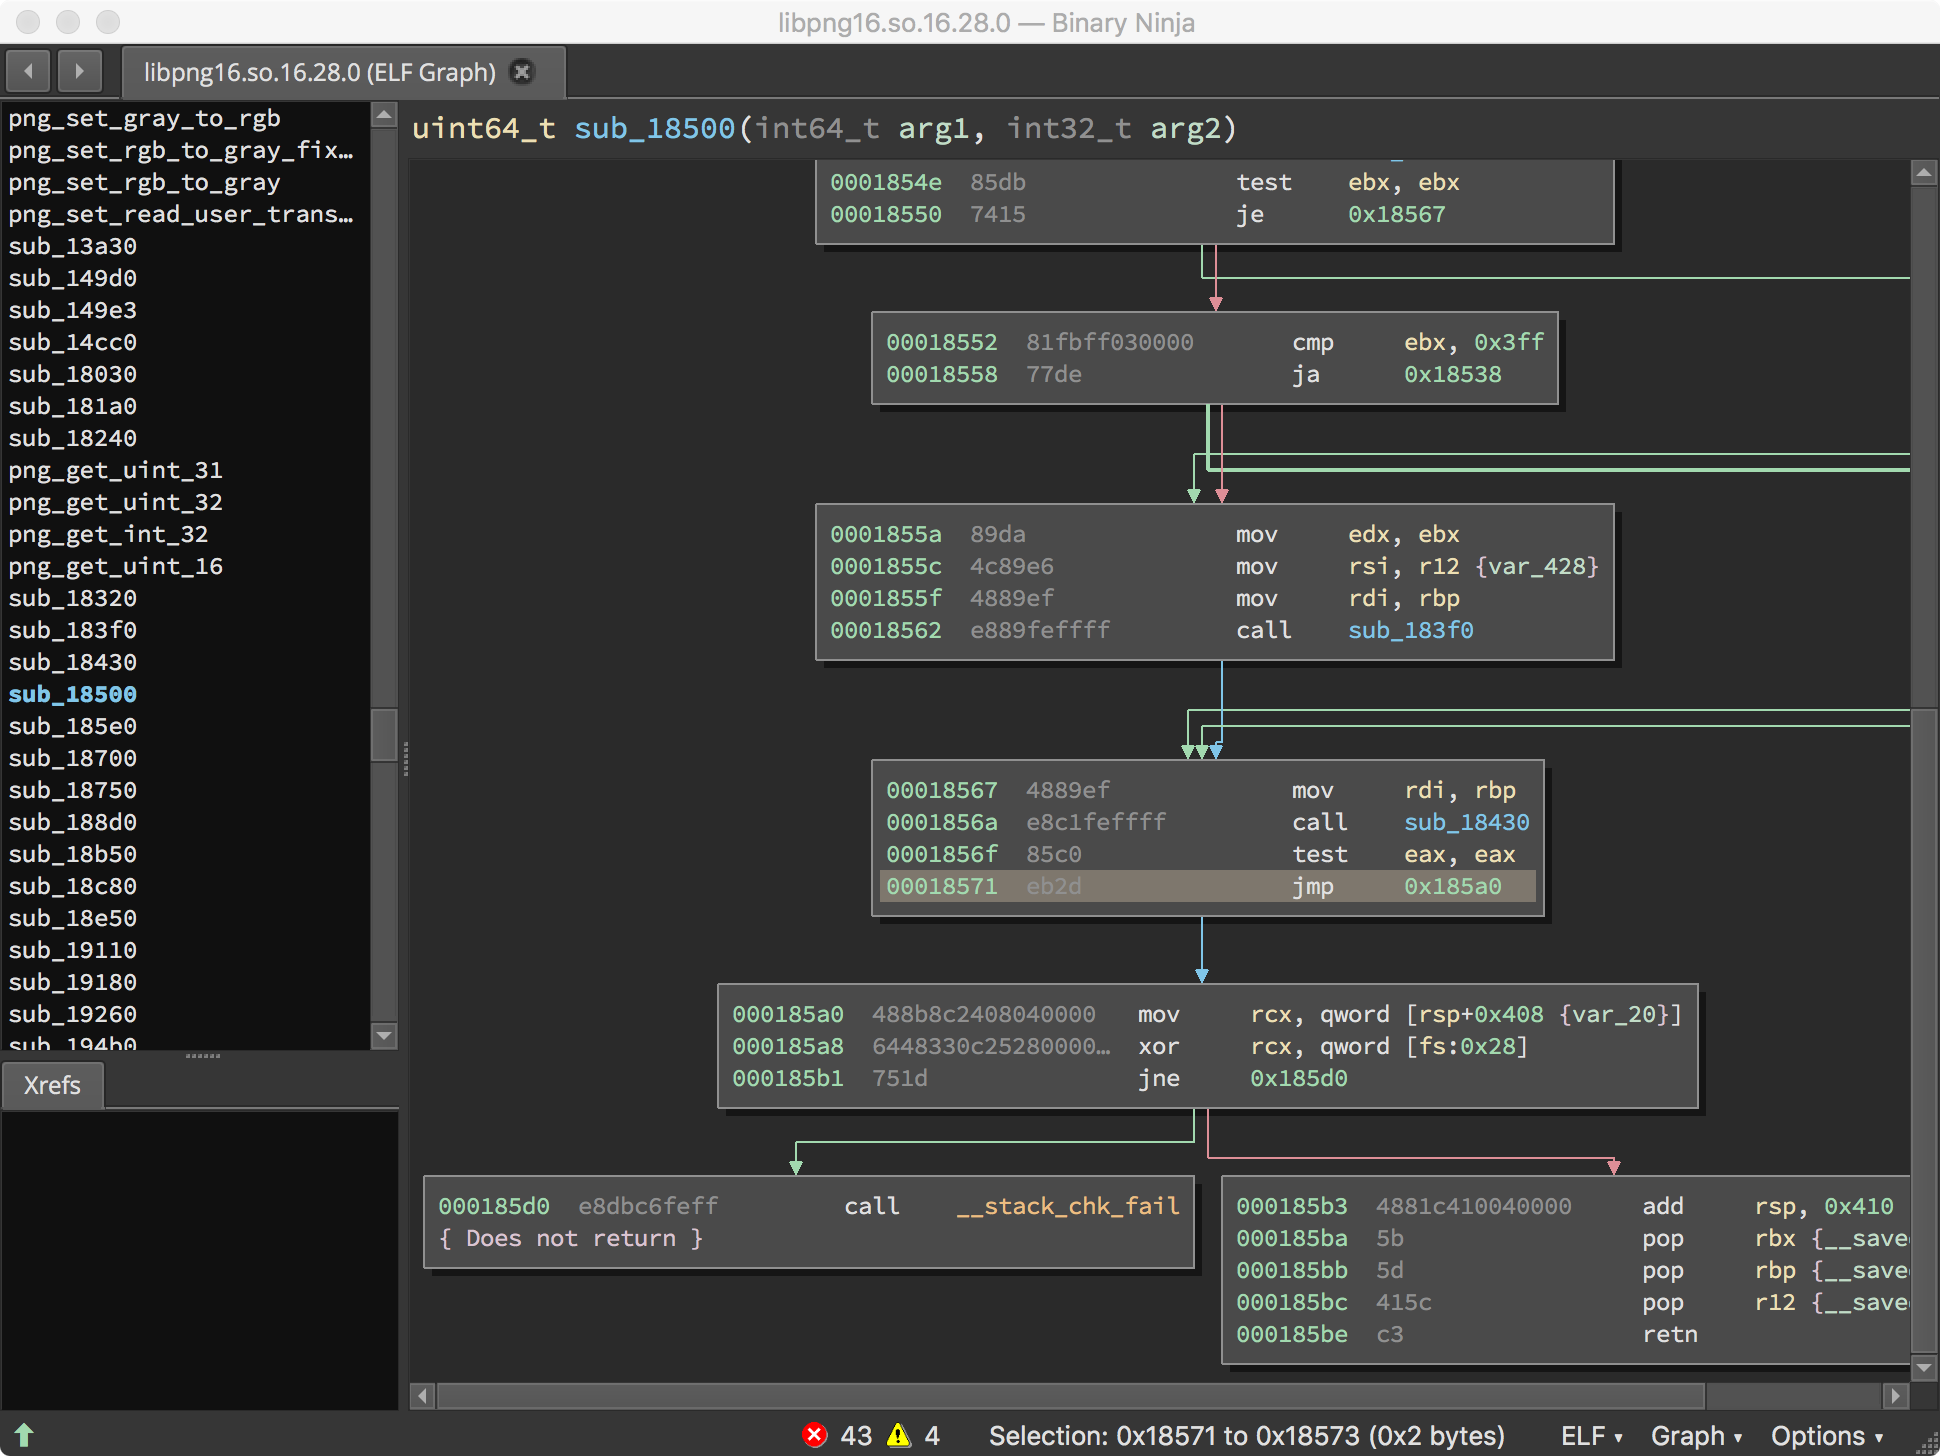
\includegraphics[width=1\textwidth]{images/imagemagick-binary-ninja-5.png}};
  \end{tikzpicture}
\end{frame}

\begin{frame}[fragile]
\frametitle{Test our patched libpng}
In Binary Ninja, go to \texttt{File -> Save Contents As}, and save your new
\texttt{lbpng.so.16.28.0}. Make sure that overwrites the original
\texttt{libpng.so}, and rerun our convert program.

\begin{lstlisting}
root@a67f5575a117:~# convert /tutorials/binary-patching/imagemagic/nsa-insignia-crc-error.png /tmp/out.png
convert-im6.q16: IDAT: CRC error `/tutorials/binary-patching/imagemagic/nsa-insignia-crc-error.png' @ error/png.c/MagickPNGErrorHandler/1628.
root@a67f5575a117:~# cp /tutorials/binary-patching/imagemagic/libpng16.so.16.28.0.patched /usr/lib/x86_64-linux-gnu/libpng16.so.16.28.0 
root@a67f5575a117:~# convert /tutorials/binary-patching/imagemagic/nsa-insignia-crc-error.png /tmp/out.png
convert-im6.q16: PNG unsigned integer out of range `/tutorials/binary-patching/imagemagic/nsa-insignia-crc-error.png' @ error/png.c/MagickPNGErrorHandler/1628.
\end{lstlisting}

Perfect! Now we don’t have to worry about imagemagick throwing out inputs just
because they have incorrect checksums.
\end{frame}


\subsection{Packaging for MAYHEM}

\begin{frame}[fragile]
\frametitle{Packaging for MAYHEM}
We can go ahead and package up this binary, and then send it off to MAYHEM for
analysis.

\begin{lstlisting}[breaklines=false]
root@a67f5575a117:~# mayhem package /usr/bin/convert -o convert
INFO:mayhem.mdbclient.commands.package:Packaging application: /usr/bin/convert
INFO:mayhem.mdbclient.commands.package:Packaging dependency: /usr/bin/convert -> convert/root/usr/bin/convert
INFO:mayhem.mdbclient.commands.package:Packaging dependency: /usr/lib/x86_64-linux-gnu/libMagickWand-6.Q16.so.3 -> convert/root/usr/lib/x86_64-linux-gnu/libMagickWand-6.Q16.so.3
INFO:mayhem.mdbclient.commands.package:Packaging dependency: /usr/lib/x86_64-linux-gnu/libMagickCore-6.Q16.so.3 -> convert/root/usr/lib/x86_64-linux-gnu/libMagickCore-6.Q16.so.3
...
INFO:mayhem.mdbclient.commands.package:Packaging dependency: /lib/x86_64-linux-gnu/libpcre.so.3 -> convert/root/lib/x86_64-linux-gnu/libpcre.so.3
INFO:mayhem.mdbclient.commands.package:Packaging dependency: /lib/x86_64-linux-gnu/libbsd.so.0 -> convert/root/lib/x86_64-linux-gnu/libbsd.so.0
INFO:mayhem.mdbclient.commands.package:Generating default configuration under: convert/config.json
INFO:mayhem.mdbclient.commands.package:Packaged /usr/bin/convert under: convert
root@a67f5575a117:~#
\end{lstlisting}
\end{frame}

\begin{frame}[fragile]
\frametitle{Packaging for MAYHEM}
We need to give MAYHEM the proper commandline invocation for \texttt{convert}.
Open \texttt{convert/config.json} with your favorite text editor, and change:

\begin{lstlisting}
"target_args": [
    "@@"
]
\end{lstlisting}

to

\begin{lstlisting}
"target_args": [
    "@@",
    "/dev/null"
]
\end{lstlisting}
\end{frame}


\begin{frame}[fragile]
\frametitle{Upload to MAYHEM}
All that’s left is uploading the package to MAYHEM!

\begin{lstlisting}
root@a67f5575a117:~# mayhem upload -u http://192.168.99.100:30128/ --start-sword convert
WARNING:mayhem.mdbclient.client:Using local environment to figure out the image
INFO:mayhem.mdbclient.commands.upload:Application successfully uploaded: 1 with harness 1
INFO:mayhem.mdbclient.commands.upload:Default job added (job_id: 1). Use that job_id to post results to the API.
\end{lstlisting}
\end{frame}

\section{Questions \& Comments}

\begin{frame}
\frametitle{Questions \& Comments}
\center{Questions \& Comments}
\end{frame}

\end{document}